\subsection{Упражнение 1}

«A Soft Murmur» — это веб-сайт, на котором можно послушать множество естественных источников шума, включая дождь, волны, ветер и т. д. 

\noindent На http://asoftmurmur.com/about/ вы можете найти их список записей, большинство из которых находится на http://freesound.org.

\noindent Загрузите несколько таких файлов и вычислите спектр каждого сигнала. Спектр мощности похож на белый шум, розовый шум, или броуновский шум? Как изменяется спектр во времени?

Возьмем два звука: пение птиц и дождь. Выделим из этих звуков короткие сегменты и построим спектры полученных сигналов.

\begin{lstlisting}[language=Python]
if not os.path.exists('28239__herbertboland__forestbirds.wav'):
    !wget https://github.com/sergeyfedorov02/Telecom/raw/main/28239__herbertboland__forestbirds.wav
    
from thinkdsp import read_wave

wave_birdsong = read_wave('28239__herbertboland__forestbirds.wav')
wave_birdsong = wave_birdsong.segment(start = 0, duration = 6)
wave_birdsong.make_audio()

spec = wave_birdsong.make_spectrum()
spec.plot_power(high = 200)
decorate(xlabel='Frequency (Hz)', ylabel='Power')
\end{lstlisting}

\begin{figure}[H]
	\begin{center}
		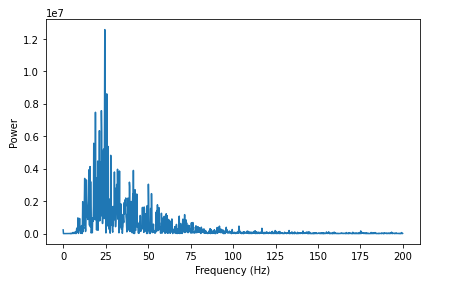
\includegraphics[scale=1]{fig/lab04/lab04_01.png}
		\caption{График сигнала}
	\end{center}
\end{figure}

Исходя из графика видно, что зависимость падения амплитуды от частоты напоминает розовый и бкелый шум (линейная зависимость). Посмотрим на спектр мощности в лагорифмическом масштабе.

\begin{lstlisting}[language=Python]
spec.plot_power()
log_birdsong = dict(xscale='log', yscale='log')
decorate(xlabel='Frequency (Hz)', ylabel='Power', **log_birdsong)
\end{lstlisting}

\begin{figure}[H]
	\begin{center}
		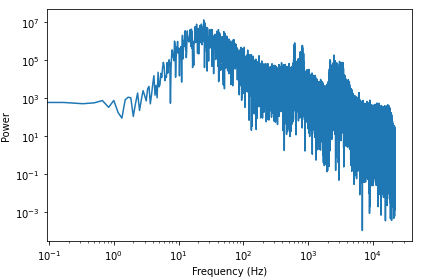
\includegraphics[scale=1]{fig/lab04/lab04_02.png}
		\caption{Спектр в логорифмическом масштабе}
	\end{center}
\end{figure}

Значение сначала возрастает, а потом уменьшается (падение удет линейно).

Рассмотрим следующий сигнал:

\begin{lstlisting}[language=Python]
if not os.path.exists('346641__inspectorj__rain-on-windows-interior-b.wav'):
    !wget https://github.com/sergeyfedorov02/Telecom/raw/main/346641__inspectorj__rain-on-windows-interior-b.wav
    
wave_rain = read_wave('346641__inspectorj__rain-on-windows-interior-b.wav')
wave_rain = wave_rain.segment(start = 0, duration = 6)
wave_rain.make_audio()

spec = wave_rain.make_spectrum()
spec.plot_power(high = 200)
decorate(xlabel='Frequency (Hz)', ylabel='Power')
\end{lstlisting}

\begin{figure}[H]
	\begin{center}
		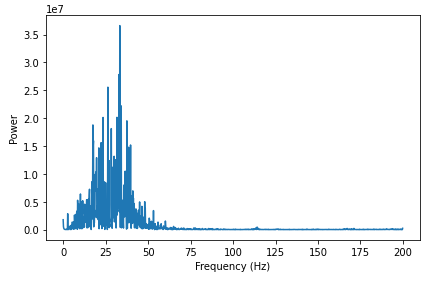
\includegraphics[scale=1]{fig/lab04/lab04_03.png}
		\caption{График сигнала}
	\end{center}
\end{figure}

Данный график также похож на предыдущий, но зависимость падения более похожа на линейную. Построим график в лагорифмическом масштабе.

\begin{lstlisting}[language=Python]
spec.plot_power()
log_rain = dict(xscale='log', yscale='log')
decorate(xlabel='Frequency (Hz)', ylabel='Power', **log_rain)
\end{lstlisting}

\begin{figure}[H]
	\begin{center}
		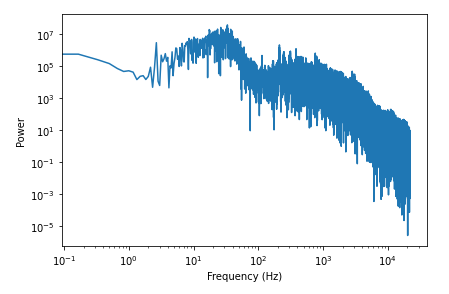
\includegraphics[scale=1]{fig/lab04/lab04_04.png}
		\caption{Спектр в логорифмическом масштабе}
	\end{center}
\end{figure}


\subsection{Упражнение 2}

Создадим метод barlet_method \cite{barlett}, который будет брать сигнал, разделять его на сегменты и вычислять спектр мощности для каждого сегмента и находить среднее по сегментам. Для этого нужно в аргументы функции сам сигнал и желаемую длину каждого сегмента. Затем вычислить спектр sp и выделить из него отдельные спектры specs. Потом выделить массив psds мощностей из каждого полученного спектра. Также вычислим среднюю мощность hs начального сигнала

\begin{lstlisting}[language=Python]
from thinkdsp import Spectrum

def barlet_method(wave, seg_length = 512, win_flag = True):
    sp = wave.make_spectrogram(seg_length, win_flag)
    specs = sp.spec_map.values()

    psds = [spectrum.power for spectrum in specs]
    hs = np.sqrt(sum(psds) / len(psds))
    fs = next(iter(specs)).fs

    return Spectrum(hs, fs, wave.framerate)
\end{lstlisting}

Проверим работоспособность функции на звуках из Упражнение 4.1

\begin{lstlisting}[language=Python]
psd = barlet_method(wave_birdsong)
psd.plot_power()
log_test_1 = dict(xscale='log', yscale='log')
decorate(xlabel='Frequency (Hz)', ylabel='Power', **log_test_1)
\end{lstlisting}

\begin{figure}[H]
	\begin{center}
		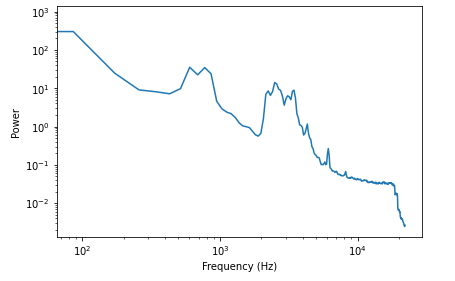
\includegraphics[scale=1]{fig/lab04/lab04_05.png}
		\caption{Результаты применения функции к первому сигналу из 4.1}
	\end{center}
\end{figure}

\begin{lstlisting}[language=Python]
psd = barlet_method(wave_rain)
psd.plot_power()
log_test_2 = dict(xscale='log', yscale='log')
decorate(xlabel='Frequency (Hz)', ylabel='Power', **log_test_2)
\end{lstlisting}

\begin{figure}[H]
	\begin{center}
		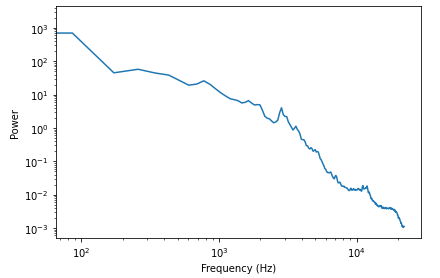
\includegraphics[scale=1]{fig/lab04/lab04_06.png}
		\caption{Результаты применения функции ко второму сигналу из 4.1}
	\end{center}
\end{figure}

Теперь зависимость между Частотой и Мощностью видна лучше, так во втором примере завимость больше похожа на линейную, как и говорилось ранее.


\subsection{Упражнение 3}

Откроем файл BTC.csv, который содержит исторические данные о ежедневной цене биткоина за последние полгода. Далее вычислим спектр цен как функцию от времени.

\begin{lstlisting}[language=Python]
if not os.path.exists('BTC_USD_2013-10-01_2020-03-26-CoinDesk.csv'):
    !wget https://github.com/AllenDowney/ThinkDSP/raw/master/code/BTC_USD_2013-10-01_2020-03-26-CoinDesk.csv
    
import pandas as pd

df = pd.read_csv('BTC_USD_2013-10-01_2020-03-26-CoinDesk.csv', parse_dates=[0])
df
\end{lstlisting}

\begin{figure}[H]
	\begin{center}
		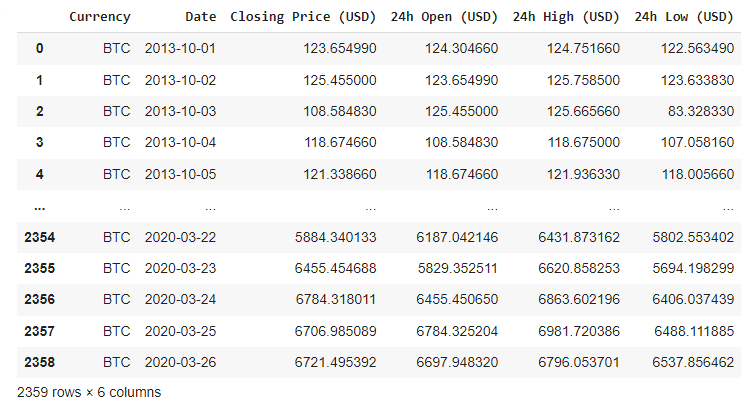
\includegraphics[scale=1]{fig/lab04/lab04_07.png}
		\caption{Таблица значений}
	\end{center}
\end{figure}

\begin{lstlisting}[language=Python]
ys = df['Closing Price (USD)']
ts = df.index

wave = thinkdsp.Wave(ys, ts, framerate = 1)
wave.plot()
decorate(xlabel='Дни')
\end{lstlisting}

\begin{figure}[H]
	\begin{center}
		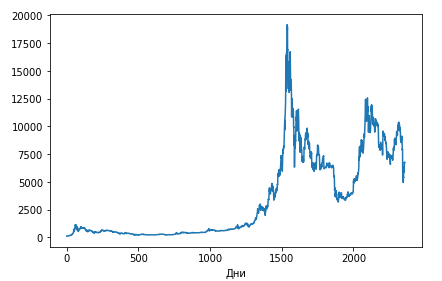
\includegraphics[scale=1]{fig/lab04/lab04_08.png}
		\caption{График цен BitCoin}
	\end{center}
\end{figure}

\begin{lstlisting}[language=Python]
spec = wave.make_spectrum()
spec.plot_power()
loglog = dict(xscale='log', yscale='log')
decorate(xlabel='Frequency (1/days)',
         ylabel='Power', 
         **loglog)
\end{lstlisting}

\begin{figure}[H]
	\begin{center}
		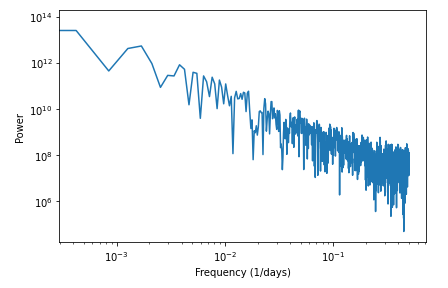
\includegraphics[scale=1]{fig/lab04/lab04_09.png}
		\caption{Спектрограмма цен BitCoin в логорифмическом формате}
	\end{center}
\end{figure}

\begin{lstlisting}[language=Python]
spec.estimate_slope()[0]

-1.7986681316517856
\end{lstlisting}

Красный шум должен иметь наклон -2. Наклон этой PSD близок к 1,7, поэтому трудно сказать, что это красным шумом или же разновидность розового шума.


\subsection{Упражнение 4}

Счетчик Гейгера — это прибор, который регистрирует радиацию. Когда ионизирующая частица попадает на детектор, он генерирует всплеск тока. Общий вывод в определенный момент времени можно смоделировать как некоррелированный шум Пуассона (UP), где каждая выборка представляет собой случайную величину из распределения Пуассона, которая соответствует количеству частиц, обнаруженных в течение интервала.

Напишем класс UncorrelatedPoissonNoise, который наследуется от класса thinkdsp._Noise, который моделирует некоррелированный пуассонвский шум (UP). Для этого следует переопределить функцию evaluate, в которой используется метод np.random.poisson(). Параметр этой функции lam - это среднее число частиц за время каждого интервала.

\begin{lstlisting}[language=Python]
from thinkdsp import Noise

class UncorrelatedPoissonNoise(Noise):
    def evaluate(self, ts):
      ys = np.random.poisson(self.amp, len(ts))
      return ys
\end{lstlisting}

Теперь сгенерируем сигнал с маленькой амплитудой(0.001) на основе этого класса. Ожидается услышать звук, как у счетчика Гейгера

\begin{lstlisting}[language=Python]
signal = UncorrelatedPoissonNoise(amp = 0.001)
wave = signal.make_wave(duration = 2, framerate = 10000)
wave.make_audio()

spec = wave.make_spectrum()
spec.plot_power()
decorate(xlabel='Frequency (Hz)', ylabel='Power', **loglog)
\end{lstlisting}

\begin{figure}[H]
	\begin{center}
		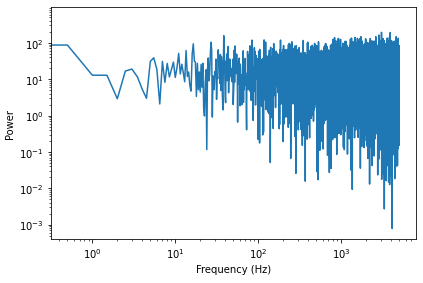
\includegraphics[scale=1]{fig/lab04/lab04_10.png}
		\caption{Получившийся спектр сигнала}
	\end{center}
\end{figure}

Теперь создадим такой же сигнал, но с большей амплитудой

\begin{lstlisting}[language=Python]
signal = UncorrelatedPoissonNoise(amp = 2)
wave = signal.make_wave(duration = 2, framerate = 10000)
wave.make_audio()

spec = wave.make_spectrum()
spec.plot_power()
decorate(xlabel='Frequency (Hz)', ylabel='Power', **loglog)
\end{lstlisting}

\begin{figure}[H]
	\begin{center}
		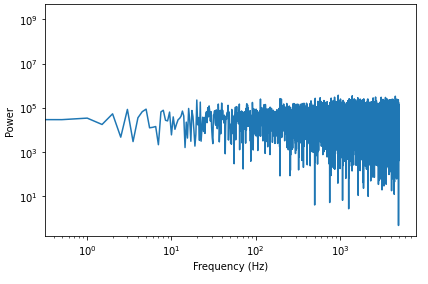
\includegraphics[scale=1]{fig/lab04/lab04_11.png}
		\caption{Получившийся спектр сигнала}
	\end{center}
\end{figure}

Результат стал похож на белый шум


\subsection{Упражнение 5}

В этой главе описан алгоритм генерации розового шума. Концептуально простой, но вычислительно затратный. Есть более эффективные альтернативы, такие как алгоритм Восса-Маккартни.

\noindent Исследуйте этот метод, реализуйте его, вычислите спектр и подтвердите, что он имеет желаемое отношение между мощностью и частотой.

Создадим функцию voss, которая реализаует более эффективный алгоритм Voss-McCartney для генерации розового шума. Вычислим спектр результата и убедимся в соответствии сотношения между мощностью и частотой.

\begin{lstlisting}[language=Python]
def voss(nrows, ncols=16):

    array = np.empty((nrows, ncols))
    array.fill(np.nan)
    array[0, :] = np.random.random(ncols)
    array[:, 0] = np.random.random(nrows)
    
    # Общее количество изменений равно nrows
    n = nrows
    cols = np.random.geometric(0.5, n)
    cols[cols >= ncols] = 0
    rows = np.random.randint(nrows, size=n)
    array[rows, cols] = np.random.random(n)

    df = pd.DataFrame(array)
    df.fillna(method='ffill', axis=0, inplace=True)
    total = df.sum(axis=1)

    return total.values
\end{lstlisting}

Проведем тестирование, для этого сгенерируем 10000 значений и превратим их в волну (построим график)

\begin{lstlisting}[language=Python]
ys = voss(10000)
ys

array([8.05587101, 6.94436007, 6.57274844, ..., 7.95820399, 8.83511144,
       8.77457504])
       
wave = thinkdsp.Wave(ys)
wave.unbias()
wave.normalize()
wave.plot()
\end{lstlisting}

\begin{figure}[H]
	\begin{center}
		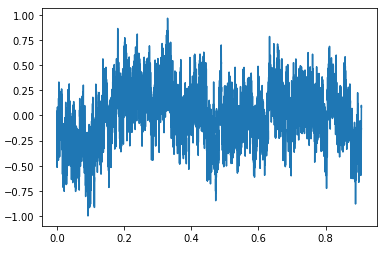
\includegraphics[scale=1]{fig/lab04/lab04_12.png}
		\caption{Сгенерированный сигнал}
	\end{center}
\end{figure}

Получился случайный звук (шум), который меньше похож на белый шум, но выглядит более случайным, чем красный шум.

Прослушаем его:

\begin{lstlisting}[language=Python]
wave.make_audio()
\end{lstlisting}

Вычислим счпектр и наклон

\begin{lstlisting}[language=Python]
spec = wave.make_spectrum()
spec.hs[0] = 0
spec.plot_power()
decorate(xlabel='Frequency (Hz)',ylabel='Power',**loglog)
\end{lstlisting}

\begin{figure}[H]
	\begin{center}
		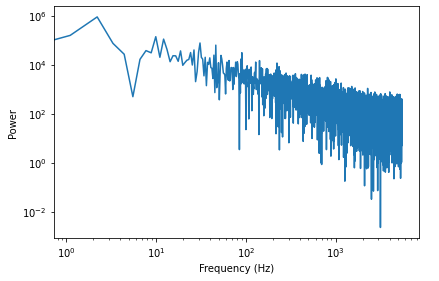
\includegraphics[scale=1]{fig/lab04/lab04_13.png}
		\caption{Спектр полученного шума}
	\end{center}
\end{figure}

\begin{lstlisting}[language=Python]
spec.estimate_slope().slope

-0.9928113664986493
\end{lstlisting}

Расчетный наклон близок к -1

Для более точной оценки сгенерируем более длинную выборку и воспользуемся методом Барлетта для вычисления среднего (найдем спектр средней мощности)

\begin{lstlisting}[language=Python]
import random

first = random.randint(50000, 70000)
first
69939

second = random.randint(100, 200)
second
129

wave = thinkdsp.Wave(voss(first * second))
spec = barlet_method(wave, seg_length=first, win_flag=False)
spec.hs[0] = 0
len(spec)
34970
\end{lstlisting}

Построим график

\begin{lstlisting}[language=Python]
spec.plot_power()
decorate(xlabel='Frequency (Hz)', ylabel='Power', **loglog)
\end{lstlisting}

\begin{figure}[H]
	\begin{center}
		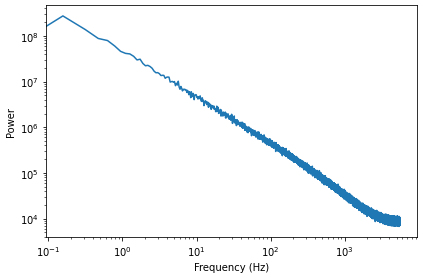
\includegraphics[scale=1]{fig/lab04/lab04_14.png}
		\caption{Спектр средней мощности шума}
	\end{center}
\end{figure}

Данный график больше похож на прямую линию, лишь с некоторой кривизной на самых высоких частотах


\begin{lstlisting}[language=Python]
spec.estimate_slope().slope

-1.0014296136950736
\end{lstlisting}

Наклон стал ближе к -1


\subsection{Вывод}

В этой работе был рассмотрен шум. Шум - сигнал, содержащий компоненты с самыми разными частотами, но не имеющий гармонической структуры периодических сигналов, рассмотреных в предыдущих работах.